\documentclass[main.tex]{subfiles}
%%------ Preamble specific to this subfile only. This will be used when this document is compiled on its own. When the main document compiles this preabble is ignored. 
%%---------------------------------------------------------------------------%

\begin{document}
\begin{frame}
  \frametitle{another frame}
  \begin{figure}[h]
    \centering
    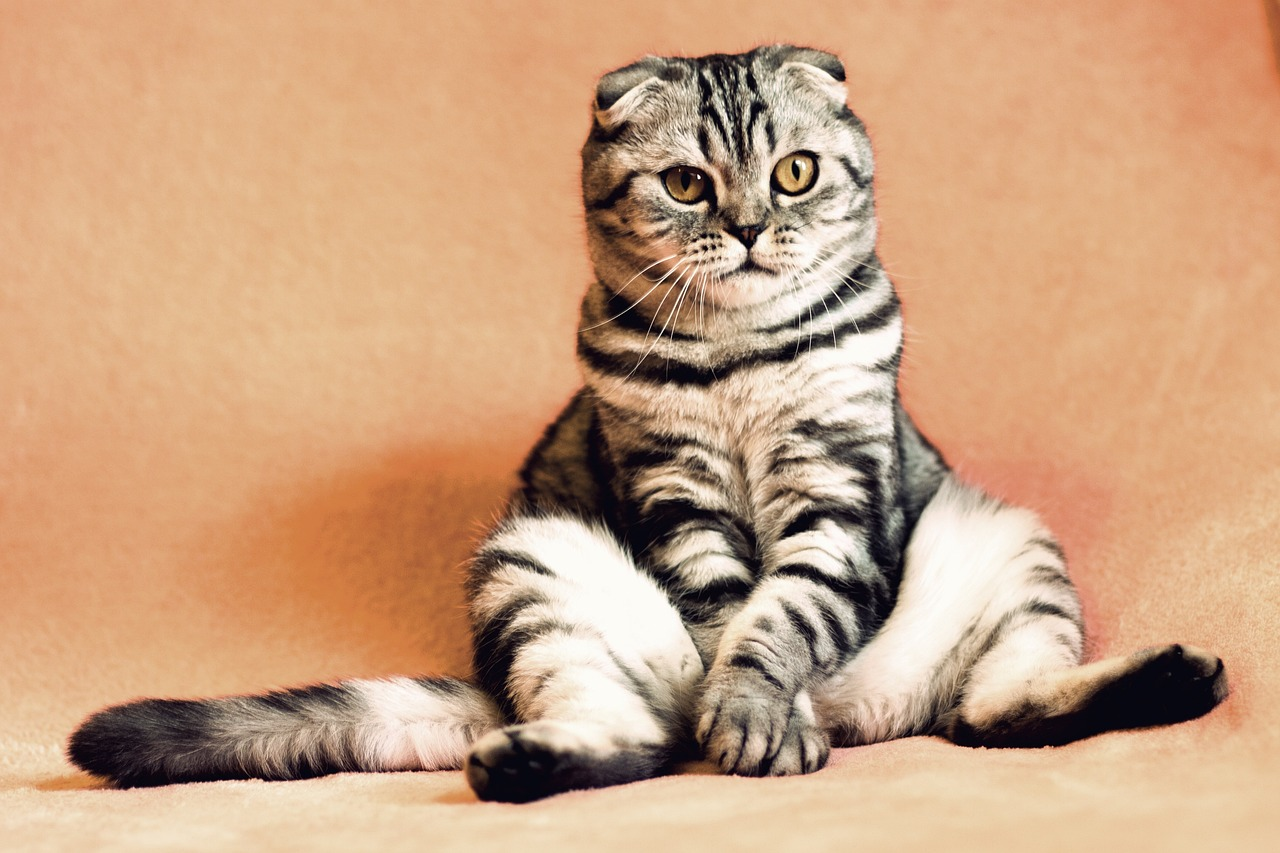
\includegraphics[width=0.3\textwidth]{cat}
    \caption{Here is a kitty!}
  \end{figure}
\end{frame}
\end{document}



% ref
%https://www.overleaf.com/learn/latex/Beamer#Adding_effects_to_a_presentation
